% 2010 年江西卷文科第 21 题：抛物线 C1、椭圆 C2 与点 Q、M、N。
% 来源 PDF：普通高考/2010/2010江西文.pdf，SHA-256 c8c86a7272df02211069e27098dcaf04a5cd8af9a9b4d54ffd14a8eb91347af3。
% 原页：第 2 页（A3 三栏）第 2 栏上部，书页码 610。
% 重绘依据：C1:x^2+y=1（开口向下、顶点 (0,1)），C2:x^2/2+y^2=1；
%   M、N 为两者在 y 轴两侧的交点，位于 y=-1/2；Q(3,1) 在右上方。
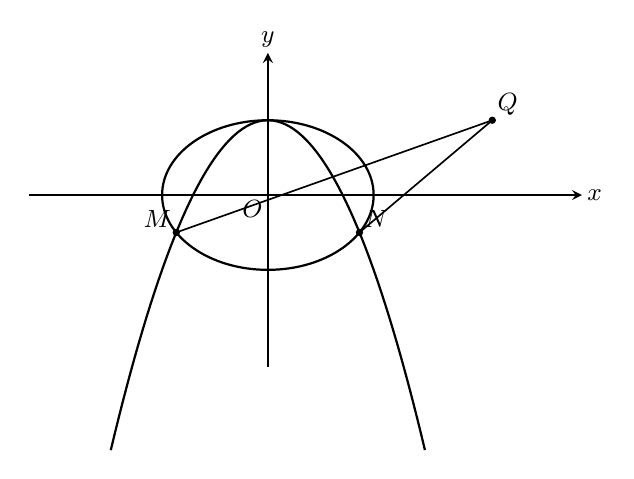
\begin{tikzpicture}[semithick, scale=0.95, every node/.style={inner sep=1.6pt, font=\small}]
  \draw[-stealth] (-3.2,0) -- (4.2,0) node[right] {$x$};
  \draw[-stealth] (0,-2.3) -- (0,1.9) node[above] {$y$};
  \draw[thick,domain=-2.1:2.1,samples=80] plot (\x,{1-(\x)*(\x)});
  \draw[thick] (0,0) ellipse (1.414 and 1);
  \fill (1.2247,-0.5) circle (1.4pt) node[above right] {$N$};
  \fill (-1.2247,-0.5) circle (1.4pt) node[above left] {$M$};
  \fill (3,1) circle (1.4pt) node[above right] {$Q$};
  \draw (3,1) -- (-1.2247,-0.5);
  \draw (3,1) -- (1.2247,-0.5);
  \node[below left] at (0,0) {$O$};
\end{tikzpicture}
